\documentclass[a4paper,10pt]{article}
\usepackage[utf8]{inputenc}
\usepackage{amsfonts}
\usepackage{tikz}
\usepackage{amsmath}
\usetikzlibrary{arrows}

\title{Telling a Story}
\author{Zongzhe Yuan}

\begin{document}

\maketitle

\section{Initial Approach to the Reduction Problem}
The discussion of the reduction problem originated from an extension of a problem that was not discussed in detail in the L11 Algebra Path Problem class. \\
In the course, we were using the algebraic approaches to represent and calculate the path problem. A path problem will be represented as a semiring and the real case to this problem will be represented and calculated by using a matrix semiring.\\
However, not all real-world problems can be solved directly with the simple matrix semiring. 
For example, when we meet the following situation (node 3 is not connected to all other nodes).\\\\
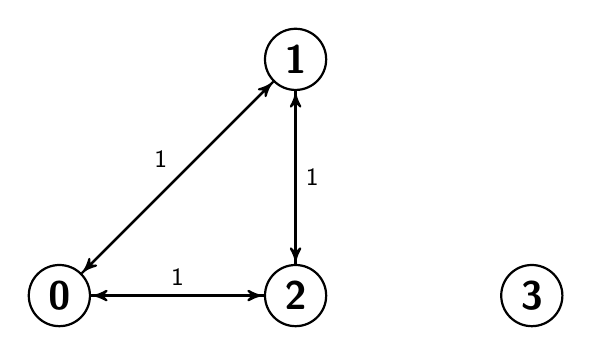
\begin{tikzpicture}[->,>=stealth',shorten >=1pt,auto,node distance=3cm,
                    thick,main node/.style={circle,draw,font=\sffamily\Large\bfseries}]

  \node[main node] (0) {0};
  \node[main node] (2) [right of=0] {2};
  \node[main node] (1) [above of=2] {1};
  \node[main node] (3) [right of=2] {3};

\path[every node/.style={font=\sffamily\small}]
    (0) edge node {1} (2)
        edge node {1} (1)
	(1) edge node {} (0)
        edge node {1} (2)
    (2) edge node {} (0)
        edge node {} (1)
;
\end{tikzpicture}\\\\
We will get the following initial path problem matrix by using the RIP protocol (here need the reference for RIP).
\[
\begin{bmatrix}
    0 & 1 & 1 & \infty \\
    1 & 0 & 1 & \infty \\
    1 & 1 & 0 & \infty \\
    \infty & \infty & \infty & 0 \\
\end{bmatrix}
\]\\
After using the RIP protocol for n-step matrix calculations, we have obtained such a matrix.
\[
\begin{bmatrix}
    0 & 1 & 1 & n+1 \\
    1 & 0 & 1 & n+1 \\
    1 & 1 & 0 & n+1 \\
    \infty & \infty & \infty & 0 \\
\end{bmatrix}
\]\\
This means that if we do not limit the number of steps in the calculation, we may get the results of the path we need in the early step (eg path from a to b), but A better solution for the entire matrix may be found after many steps (or the calculation will counting to infinity, which is shown in the previous example).\\\\
Thus, in the course L11, instead of using RIP and simple matrix semiring approach, we used another protocol called BGP (here need the reference for BGP). We start from the simple $(\mathbb{N},min,+)$ semiring that calculate the shortest distance, and we use lexicographic product (need reference to the Background/Definition) to construct a new semiring that contains the shortest-path metric and the set of its path.\\\\
(these definition could be moved into definition section)\\
Here we need to define some new operators/new rules for our semigroup:\\
Assume $(S,\bullet)$ is a semigroup. Let $lift(S,\bullet)\equiv (fin(2^S),\hat\bullet)$ where
$X \hat\bullet Y = \{x\bullet y |x\in X,y\in Y\}$.\\
Then we can use our $lift$ to construct a bi-semigroup:\\
Assume $(S,\bullet)$ is a semigroup. Let $union\_lift(S,\bullet)\equiv (\mathcal{P}(S),\cup,\hat\bullet)$ where
$X \hat\bullet Y = \{x\bullet y |x\in X,y\in Y\}$, and $X,Y \in \mathcal{P}(S)$, which is the set of finite subsets of $S$.\\
Then for a given graph $G = (V,E)$, we define $path(E)\equiv union\_lift(E^*,.)$ where . is the concatenation function of sequence.\\
Finally we get our "shortest paths with paths" semiring from a given graph $G = (V,E)$: $spwp \equiv AddZero(\bar0,(\mathbb{N},min,+) \overrightarrow{\times} path(E))$.\\\\
Here comes to the problem, when we are using spwp for calculations, because there may have loops in our $path(E)$, we need a lot of extra computation (though it will eventually yield correct results) to prove that the paths that have loops are not the shortest path.
Therefore, in order to eliminate these paths with loops, we have introduced a new concept in the L11 course, Reduction.\\\\
If $(S,\oplus,\otimes)$ is a semiring and $r$ is a function from $S$ to $S$, then $r$ is a reduction if $\forall a,b \in S$, $r(a) = r(r(a))$, $r(a\oplus b) = r(r(a)\oplus b) = r(a\oplus r(b))$ and 
$r(a\otimes b) = r(r(a)\otimes b) = r(a\otimes r(b))$.\\
So, if $(S,\oplus,\otimes)$ is a semiring and $r$ is a reduction, then $red_r(S) = (S_r,\oplus_r,\otimes_r)$, where $S_r = \{s\in S|r(s)= s\}$, $x\oplus_r y = r(x\oplus y)$ and $x\otimes_r y = r(x\otimes y)$.\\
Hence we return to our path problem. Fro a given path $p$, we say $p$ is elementary if there is no node inside $p$ that is repeated. Then we can define our elementary path using the reduction $r(X) = \{p\in X | p $ is elementary$\} $ and $epaths(E) = red_r(paths(E))$.\\\\
Therefore, our path problem semiring becomes to $AddZero(\bar0,(\mathbb{N},min,+) \overrightarrow{\times} epath(E))$.\\\\
However, we still encounter the problem that an element in the matrix that has a path distance value but does not have edges in its path. So we need to define a second reduction, which turns all elements that don't satisfy the condition into a single element (the zero we added into our semiring).\\
$r_2 (inr(\infty)) = inr(\infty)$, $r_2 (inl(s,\{\})) = inr(\infty)$ and $r_2 (inl(s,W)) = inl(s,W)$ where $W$ is not empty.
Therefore, our path problem semiring becomes to $red_{r_2}(AddZero(\bar0,(\mathbb{N},min,+) \overrightarrow{\times} epath(E)))$.\\\\
It is worth mentioning that we did not discuss the properties of reduction in detail in the L11 course. We also did not know whether the original semiring still satisfies the semiring property after the reduction. At the same time, the properties of some of the original operators (such as commutative rules) remains after reduction or not is also a mystery to us.\\
These are the topics that we need to focus our discussion on.
It is worth mentioning that the first reduction (reduce all pathes that are not elementary) that we defined above does not follow the property of the reduction we defined for reduction on the $min$ operation. Imagine we have path $B = \{a,b,c,d\}$ that is longer but does not have loop and $B = \{a,b,b\}$ that is shorter but does have loop. Then $r(A\oplus B) = r(B) = \infty$ because $B$ is shorter but has loop, but $r(A\oplus r(B)) = r(A \oplus \infty) = r(A) = A$ because $B$ has loops but $A$ doesn't.\\
Therefore, we not only discuss the properties of reduction, but also try to find another way to represent reduction to solve the problem of our path problem.
\section{Classical Reduction and Example}
In order to better understand reduction and further analyze it in detail, we trace the source to find out if there is any other definition and study of reduction before us. 
In fact, the earliest definition we could find about reduction came from Ahnont Wongseelashote in 1977\cite{WONGSEELASHOTE197955}. Wongseelashote also encountered the problem similar to ours when studying the path problem in the paper. In fact, our definition of reduction is very similar to Wongseelashote's definition of reduction (the real reason is that L11 refers to the Wongseelashote definition when defining reduction). However, unfortunately, Wongseelashoth only put forward the concept of reduction in the paper without detailed reasoning and structure proof.\\
Next we found that Alexander James Telford Gurney also mentioned the concept of reduction in his Ph.D thesis\cite{gurney_construction_2010}. Gurney's discussion of reduction is also based on the definition by Wongseelashote, and it also does not focus on reduction for detailed structure proof.\\\\
Therefore, we can temporarily use the previously mentioned definition of reduction as “classical reduction” and reasoning (because it does not satisfy our elementary path problem and is extraction and implementation un-friendly, so we call it classical).\\
To help us understand reduction and study its properties, we found another example of reduction in the course of L11.\\\\
The reduction is call $min_{\leq}$ (Martelli’s semiring)\cite{martelli_gaussian_1976} which means remove all the superset.
For a given graph $G = (V,E)$, A cut set $C \in E$ for nodes $i$ and $j$ is a set of edges such there is no path from $i$ to $j$ in the graph $(V, E - C)$. $C$ is minimal if no proper subset of $C$ is a cut set. And Martelli’s semiring is such that $A^{(*)}(i, j)$ is the set of all minimal cut sets for $i$ and $j$. 
So Martelli’s semiring =$(S,\oplus,\otimes,\bar0,\bar1)$ where $S = min_\leq(2^{2^E})$, $X\oplus Y = min_\leq(\{U \cup V | U \in X, V \in Y\})$, $X\otimes Y = min_\leq(X \cup Y)$, $\bar0 = \{\{\}\}$ and $\bar1 = \{\}$.\\
Here we can easily prove that $min_\leq$ satisfies our previous definition of reduction. So $min_\leq$ is a classical reduction. (I am considering whether or not paste the proof of matrelli's semiring)
\section{Generalized Reduction}

\section{Predicate Reduction}
\section{Construct the Path Problem Semiring}

\medskip

\bibliographystyle{unsrt} 
\bibliography{MphilProject}

\end{document}
